\documentclass[12pt,a4paper]{article}

% Paquetes básicos
\usepackage[utf8]{inputenc}
\usepackage[spanish]{babel}
\usepackage{graphicx}
\usepackage{xcolor}
\usepackage{amsmath}
\usepackage{amssymb}
\usepackage{hyperref}
\usepackage{geometry}
\usepackage{listings}
\usepackage{xcolor}
\usepackage{float}
\usepackage{epigraph}
\usepackage{cite}

% Configurar márgenes
\geometry{
    top=2.5cm,
    bottom=2.5cm,
    left=3cm,
    right=3cm
}

% Información del documento
\title{Diseño del modelo multidimensional utilizando las fases del modelo de Kimball\\
\large - AAPAD - }
\author{Marcelo Ferreiro Sánchez\\ Pablo Chantada Saborido \\ Gillermo García Engelmo \\Pepe Romero Conde}
\date{\today}

\begin{document}

\maketitle

\tableofcontents

\newpage

\section{Introdución}

No presente informe descríbese o diseño da nosa Base de Datos Analítica. \\


Nós somos parte do equipo técnico de Airbnb e para analizar o negocio e evaluar onde pode mellorarse ou que aspectos estan a fallar encomendóusenos o diseño dunha Base de Datos Analítica. Se ben os directivos facilitaronnos unhas preguntas ás que queren respostas (\emph{consultas} na nosa Base de Datos) tamén temos que satisfacer a restriccións dos datos en si mesmos. Non podemos simplemente diseñar o Almacén de datos que queramos, ten que ser posible chegar a él a partires dos \texttt{.csv} que temos a nosa disposición. Polo tanto a nosa aproximación metódoloxica é hibrida, pois dispoñemos de restriccións de \textbf{ o proceso de negocio} a modelar (de alto nivel, materializadas nas \emph{consultas}) e de \textbf{as fontes de datos} (baixo nivel, materializadas nos \texttt{.csv}). 


\section{Restricións}
\subsection{Proceso de negocio, parte \emph{top-down}}

O interés desde o punto de vista de o proceso de negocio e respostar a: as preguntas evidentes facilmente formulables e ás preguntas que xurdan en función destas. Por eso, polo que poda ocurrir elixiremos sempre a granularidade máis pequena (ver sección 3.2). 

\subsubsection{Consultas}

\begin{itemize}
	\item Teñen mellores valoracións os terratenentes con múltiples vivendas? (HOSPEDADOR, score)
	\item Canta é a influencia dos axentes externos no número de reservas? (TEMPO, EVENTOS, CHUVIA)
	\item Inflúe a idade do arrendatario no seu calendario de viaxes? (VALORADOR, TEMPO)
	\item Que caracteriza ós arrendatarios con máis valoracións feitas? (VALORADOR)
	\item Que caracteriza ós arrendadores con mellores \emph{scores}? (HOSPEDADOR, verificacións)
	\item Como é a relación entre o precio e o score? Os barrios máis caros teñen mellores scores? (HOSPEDAXE, LOCALIZACIÓN)
	\item Depende o número de verificacións do tempo de resposta? (HOSPEDADOR)
	\item Que amenities correlacionan con mellores scores? (AMENITY, HOSPEDAXE)
	\item Varía a importancia das amenities por localización ou temporada? (AMENITY, LOCALIZACIÓN, TEMPO)
\end{itemize}

\subsection{Fontes de datos, parte \emph{bottom-up}}

Veúsenos dado, como punto de partida material para o desenvolvemento do Almacén de Datos, unha colección de \texttt{.csv}s, nos que, para cada cidade dispoñemos do seguinte (ver Figura \ref{fig:oltp}):
\begin{itemize}
	\item \texttt{hospedaxes}: cada fila é un obxecto de aluguer. Tense información de valor \footnote{acompañada de información que non aporta ó análise do negocio.} sobre: os donos (quenes son e información sobre eles); cantos baños, habitacións e dormitorios hai; cantas persoas poden alugar; o barrio; a dispoñibilidade e información xeral de reserva (cantas noites como mínimo); puntuación das valoracións; e as \textbf{amenities} (formato JSON array).
	\item \texttt{hospedaxes\_resumo}: é un subconxunto das columnas de \texttt{hospedaxes}. Por tanto máis manexable pero sin información adicional.  
	\item \texttt{calendario}: ten un rexistro da dispoñibilidade de os hospedaxes ó largo do tempo. Seranos de utilidade para caracterizar a influecia de factores externos.
	\item \texttt{valoracions}: dinos \emph{quen} fixo \emph{que} reseña e \emph{cando}. No proceso ETL estas reseñas deberan sufrir un proceso de conversión a través dunha ferramenta de Procesamento da Linguaxe Natural (NLP) para obter un \emph{score} númerico, máis útil á hora de ser agregado que a reseña en si mesma.
	\item \texttt{valoracions\_resumo}: son pares (\texttt{id\_hospedaxe}, \texttt{data}).
	\item \texttt{vecindario}: Esta táboa dependendo da cidade da que a descarguemos, pode conter unha pequena información do barrio ou estar baleira directamente. No que sigue, simularemos a súa completitude con información aleatoria, por cuestións do alcance da práctica.
	
\end{itemize}

\textbf{Nota:} As \texttt{amenities} e \texttt{host\_verifications} son campos multivaluados en formato array que requiren procesamento no ETL. As reviews individuais con data e reviewer provén de \texttt{reviews.csv}.

\begin{figure}[h!]
  \centering
  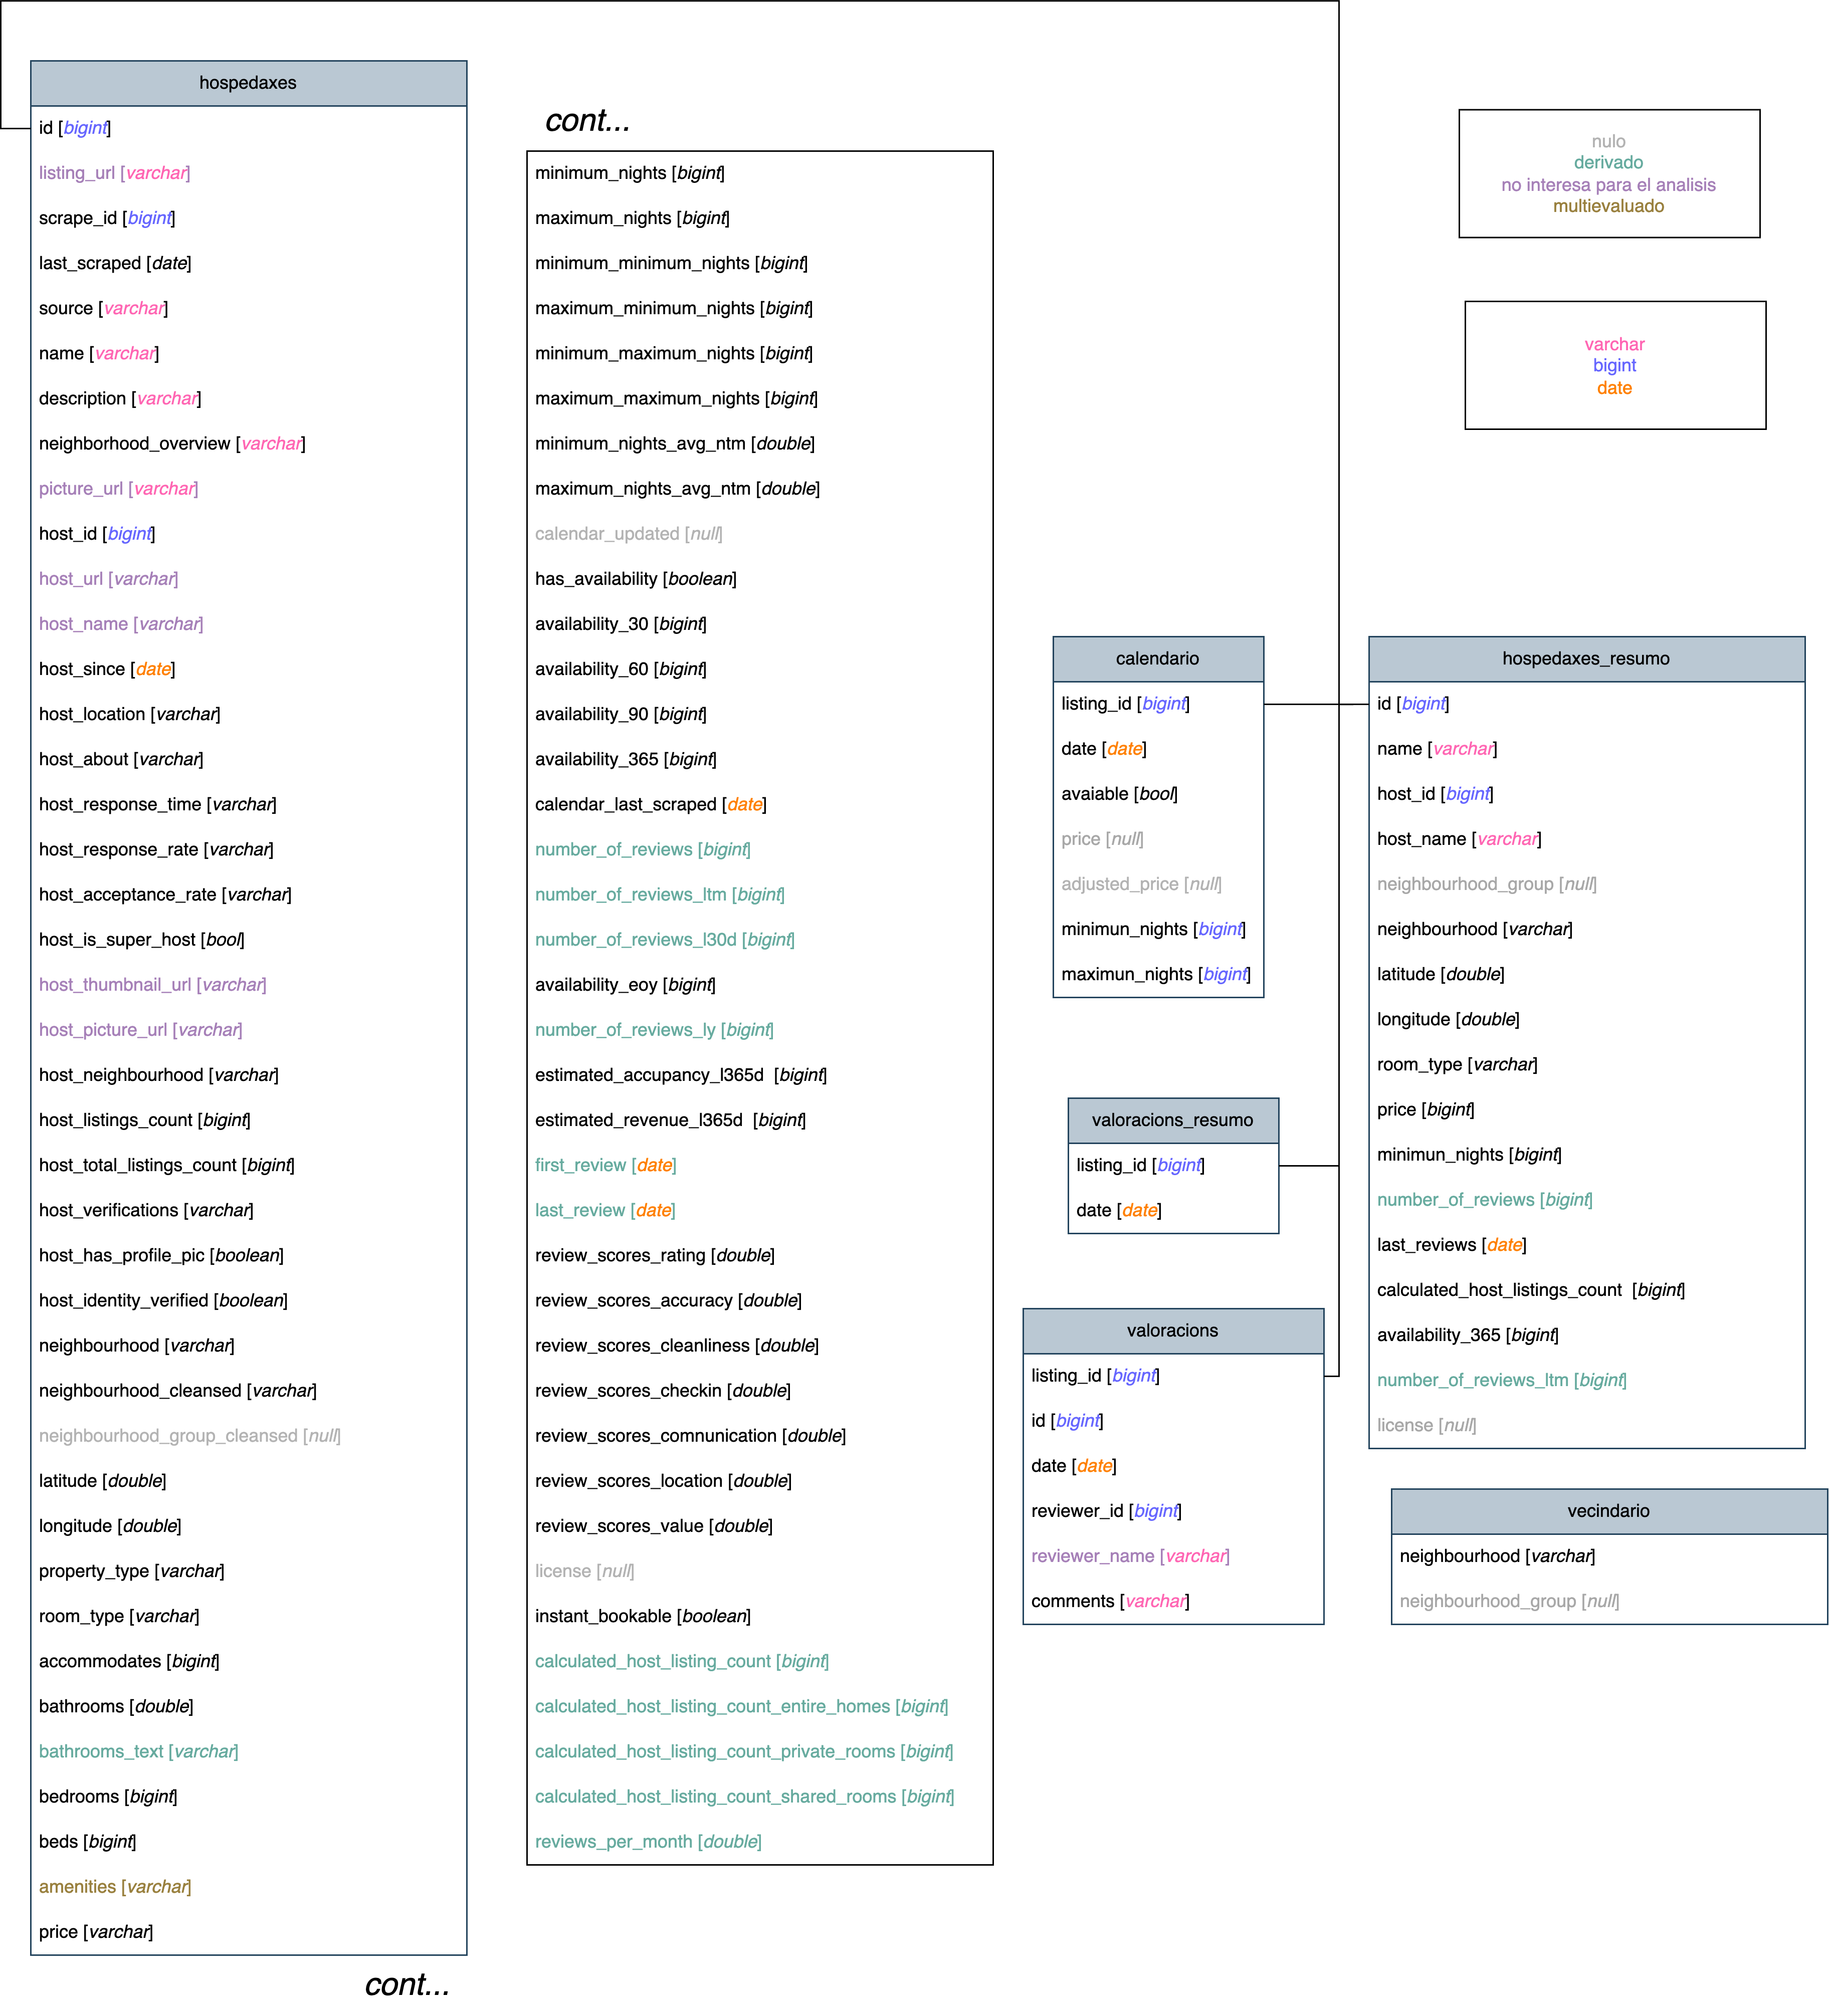
\includegraphics[width=\textwidth]{diagramas/antes.drawio.png}
  \caption{Diagrama de los datos del OLTP}
  \label{fig:oltp}
\end{figure}

\subsection{Suposiciones adicionales}

Para a futura construcción da Base de Datos Analítica serán precisas as seguintes fontes de información actualmente non dispoñibles (para o complimento da práctica é probable que inventemos os datos):
\begin{itemize}
	\item Información adicional sobre os arrendatarios (actualmente só dispoñemos o nome). Idealmente deberíamos contar con: fecha de nacemento, xénero, lugar de nacemento...
	\item Rexistros meteorolóxicos (chuvia, neve, altas temperaturas). Estos datos integraranse naturalmente no modelo dimensial como unha dimensión máis.
	\item Información sobre eventos de interese tales comos concertos de música ou partidos deportivos.
\end{itemize}

\section{Detalles da implementación}

A continuación descríbese as decisións técnicas que tiveron lugar na construcción do Modelo de Feitos Dimensionais. Para unha representación visual ver a Figura \ref{fig:dfm}.

\begin{figure}[h!]
  \centering
  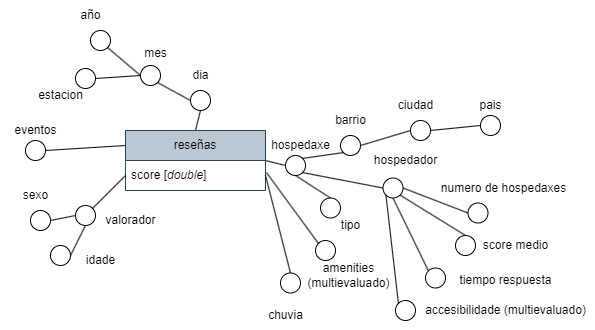
\includegraphics[width=\textwidth]{diagramas/multidimensional.drawio.png}
  \caption{Diagrama do Modelo de Feitos Dimensional (\emph{DFM}). Nota: A dimensión AMENITY conecta con HOSPEDAXE mediante relación N:M a través dunha táboa ponte. Atributos: amenity\_id, nome, categoría.}
  \label{fig:dfm}
\end{figure}

\subsection{Qué é cada cousa?}

No noso modelo as reseñas son os \textbf{feitos}, pois son moitos e crecen a moita velocidade, e son un punto de partida para moitos análisis. É posible que cada departamento teña as súas necesidades especiais, e eventualmente poderase crear \emph{data marts} para cada un deles, pero nós pensamos que as reseñas son de alto interés para calqueira análise. Estas contan cunha única \textbf{métrica}, o \emph{score}, que indica o grao de satisfacción do usuario ca experiencia do hospedaxe. Así, as circunstancias que circumbalan á reseña son ás \textbf{dimensións}, responden as seguintes preguntas:
\begin{itemize}
	\item \emph{Quen?} O valorador, cos seus atributos: idade, sexo.
	\item \emph{Cando?} Indicando ate o día, con información de estacións (para estudar a influencia da tempada alta).
	\item \emph{A que?} O hospedaxe. Este á sua vez debe respostar a: \emph{De quen?} (o propietario, cos seus atributos) e \emph{Onde?} (localización).
	\item \emph{Que amenities?} Comodidades do hospedaxe (Wifi, cocina, piscina...) mediante táboa ponte N:M.
	\item \emph{Baixo que circunstancias?} Información meteorolóxica e de eventos xerais.
\end{itemize}

Pódese apreciar que dentro de \emph{A que?} vai \emph{De quen?} e \emph{Onde?}. Esto indica que o noso Modelo sigue os esquema de copo de neve \cite{kimball1996}, xustificado por evitar redundancia (un hospedador ten múltiples hospedaxes) e implementar xerarquías xeográficas eficientemente. O trade-off é máis JOINs nas consultas, aceptable para un DW analítico.

\subsection{Granularidade}

\epigraph{
"All grain definitions should start at the lowest, most atomic grain and should describe the physical process that collects the data."
}{
Ralph Kimball \cite{kimball2007}
}

No noso diseño levamos a granularidade ó máis fino que podemos: as datas van ate o día, os lugares ate os barrios, e cada fila da táboa de feitos representa unha \textbf{reseña individual}. Esta granularidade atómica permite máxima flexibilidade nas consultas analíticas.

\subsection{Dimensións particulares}

\subsubsection{Dimensións dexeneradas}

Non temos dimensións dexeneradas. Todas as dimensións (TEMPO, VALORADOR, HOSPEDAXE, HOSPEDADOR, LOCALIZACIÓN, AMENITY, EVENTOS, CHUVIA) contan con táboas propias e atributos descritivos.

\subsubsection{Atributos multivaluados}

\textbf{AMENITIES:} Nos datos fonte aparecen como array JSON: \texttt{["Wifi", "Kitchen", "TV"]}. Implementamos unha táboa ponte (bridge table):

\begin{center}
HOSPEDAXE $---<$ HOSPEDAXE\_AMENITY $>---$ AMENITY
\end{center}

Táboa AMENITY: \texttt{amenity\_id} (PK), \texttt{nome}, \texttt{categoría}. \\
Táboa HOSPEDAXE\_AMENITY: \texttt{hospedaxe\_id} (FK), \texttt{amenity\_id} (FK).

Xustificación: alta cardinalidade (50-200+ valores únicos), crecemento dinámico, permite consultas flexibles. No ETL parseamos o JSON, normalizamos nomes e poboamos as táboas. Ao agregar, úsase \texttt{COUNT(DISTINCT)} para evitar duplicación.

\textbf{HOST\_VERIFICATIONS:} Array como \texttt{['email', 'phone', 'work\_email']}. Desnormalizamos en atributos booleanos na táboa HOSPEDADOR: \texttt{email\_verificado}, \texttt{telefono\_verificado}, \texttt{work\_email\_verificado} (CHAR(1): 'S'/'N'). Xustificación: baixa cardinalidade (4-5 valores), simplifica consultas, valores estables.

\subsubsection{Dimensións basura}

Non identificamos dimensións basura no modelo.

\subsubsection{Dimensións que cambian no tempo (SCD)}

\textbf{HOSPEDADOR e HOSPEDAXE:} SCD Tipo 1 (sobrescribir). Atributos como \texttt{score\_medio}, \texttt{tempo\_resposta}, \texttt{price} cambian, pero para análise de reviews interésanos o estado actual. Cada review é un snapshot puntual, manter histórico completo (Tipo 2) complicaría o modelo sen valor analítico significativo.

\textbf{LOCALIZACIÓN, TEMPO, EVENTOS, CHUVIA, AMENITY:} SCD Tipo 0 (sen cambios). Son datos estables ou históricos.

\textbf{VALORADOR:} SCD Tipo 1. A idade calcúlase da data de nacemento.

\subsubsection{Xerarquías dimensionais}

\begin{itemize}
	\item TEMPO: día $\rightarrow$ mes $\rightarrow$ ano; día $\rightarrow$ estación $\rightarrow$ ano
	\item LOCALIZACIÓN: barrio $\rightarrow$ cidade $\rightarrow$ país
	\item VALORADOR: idade $\rightarrow$ grupo\_etario (18-25, 26-35, 36-50, 51+)
	\item AMENITY: nome $\rightarrow$ categoría
\end{itemize}

\subsection{Métricas}

A nosa métrica principal é o \textbf{SCORE} (DECIMAL(3,2), rango 0.00-5.00).

\textbf{Carácter: NON ADITIVA.} Non se pode sumar: $\frac{3}{5} + \frac{4}{5} = \frac{7}{5}$ non ten sentido semántico. As valoracións miden satisfacción nunha escala fixa, non son magnitudes acumulables.

\textbf{Operacións válidas:}
\begin{itemize}
	\item \texttt{AVG(score)}: agregación principal por hospedaxe, barrio, hospedador, estación, amenity
	\item \texttt{COUNT(*)}: volume de reviews (ADITIVA)
	\item \texttt{COUNT(DISTINCT valorador\_id)}: usuarios únicos (ADITIVA)
	\item \texttt{MIN/MAX/MEDIAN/STDDEV(score)}: rangos e distribucións (NON ADITIVAS)
\end{itemize}

Métricas derivadas: contaxes (aditivas), agregacións de score (non aditivas), proporcións (non aditivas).

\newpage

\bibliographystyle{plain}
\bibliography{referencias}


\end{document}